\documentclass[rnd]{mas_proposal}
% \documentclass[thesis]{mas_proposal}
\usepackage[utf8]{inputenc}
%\DeclareUnicodeCharacter{25CF}{$\bullet$}
%\DeclareUnicodeCharacter{251C}{\mbox{\kern.23em
%  \vrule height2.2exdepth1exwidth.4pt\vrule height2.2ptdepth-1.8ptwidth.23em}}
%\DeclareUnicodeCharacter{2500}{\mbox{\vrule height2.2ptdepth-1.8ptwidth.5em}}
%\DeclareUnicodeCharacter{2514}{\mbox{\kern.23em
%  \vrule height2.2exdepth-1.8ptwidth.4pt\vrule height2.2ptdepth-1.8ptwidth.23em}}
\usepackage{amsmath}
\usepackage{amsfonts}
\usepackage{amssymb}
\usepackage{graphicx}
%\usepackage{cite}
\usepackage{hyperref}
\hypersetup{%
   colorlinks=true,
   citecolor=black,
   colorlinks=false,
   linkcolor={black},
   raiselinks=false
  }
  
\title{Evaluation of Active Learning for Short Answer Grading}
\author{Mohandass Muthuraja, Jeeveeswaran Kishaan}
\supervisors{Prof. Paul G. Ploeger\\Deebul Nair }

% \thirdpartylogo{path/to/your/image}

\begin{document}

\maketitle

\pagestyle{plain}

\chapter{Introduction}

\vspace{4mm}
 
Assessment of the knowledge acquired by the students is one of the most important aspects of the learning process. Different forms of assessments that exist today include multiple choice questions, fill-in-the-blanks, essay questions and short answer questions. Prior works have shown that multiple choice questions and fill-in-the-blanks fail to capture the vital aspects of the acquired knowledge such as reasoning and self-explanation \cite{Wang2008}. In contrast, questions which require the students to construct responses in natural language have been found to be more effective in assessing their grasp on the subject matter \cite{Roy2016a}. Essay questions and short answer questions belong to this category.  

\vspace{4mm}

Limited availability of teachers, online learning platforms, and individual or group study sessions done outside classrooms necessitated quick and efficient assessment of free text responses. Computer assisted assessment / automatic grading evolved as a solution to this problem and a lot of research has been done on automating the grading of essay\cite{Higgins2004} and short answer responses\cite{Leacock2003, Pulman2005, Mohler2009}. The focus of this work would be on improving the existing solutions to grade short answer questions. Short answer questions are characterized by the following aspects\cite{Burrows2015}:

\begin{itemize}

\item the question must require a response that recalls external knowledge instead of requiring the answer to be recognized from within the question

\item the question must require a response given in natural language

\item the answer length should be roughly between one phrase and one paragraph

\item the assessment of the responses should focus on the content instead of writing style

\item the level of openness in open-ended versus close-ended responses should be restricted with an objective question design 

\end{itemize}

Automatic short answer grading essentially deals with using computational methods to predict the grades for students' answers, thus cutting down the effort and time of teachers / professors. Many automated approaches have been proposed in the past for grading short answer questions. These methods compare how similar the students' answers are to the one provided by the teacher or professor and assign a grade proportional to the magnitude of similarity \cite{Mohler2011}. Different approaches of computing these similarity measures include handcrafted pattern matching, automatic pattern matching, lexical similarity (how particular words effect other words), semantic similarity (deals with the meaning of sentences), and entailments (whether one sentence leads to another without any contradiction). Fig \ref{auto_workflow} shows a general workflow of automatic short answer grading as a pipeline. After creating a dataset of all the students' answers and model answers written by the teachers, useful features are extracted from the answers using natural language processing techniques. A model is developed based on these features and it is evaluated on new datasets.

\vspace{3mm}

\begin{figure}[h!]
	\includegraphics[width=\textwidth]{images/autograding_workflow}
	\caption{Workflow of automatic short answer grading \cite{Burrows2015}.}
	\label{auto_workflow}
\end{figure}

All the above-mentioned methods belong to a learning paradigm called supervised learning where the right answer for every question is available \cite{Horbach2016}. Though these approaches were able to produce decent results, they suffer from many shortcomings such as;

\begin{itemize}

\item the failure to capture the different wordings/phrasing of the students while trying to answer the short answer questions. It is obvious that anticipating all different ways of answering his questions is practically impossible for the professor. 

\item lack of sufficient amount of labeled training data in the domain to learn the models. Reasons include privacy, availability, and the quality of the correct answers. 

\item inability to capture consistent patterns of misunderstandings among students. Ability to recognize such patterns would enable the automated systems to provide useful feedback to students as to why there was a reduction in marks awarded.

\item accounting for small deviations in the answers which might affect the whole meaning of the sentence (for ex. in mathematical terms, though each and every word of the student's answer align with that of the professor, a small negation or inverse operation would change the whole meaning).

\item finding a way to understand the underlying concept of various students' answers and bagging the similar ones (or the right and wrong ones separately) is also a very tedious task. 

\item being a passive learner, these models learn the rules once and apply them on new input answers. Thus, it would be very difficult to achieve robustness when applied to new data over time. \\

\end{itemize}

This work proposes an approach where a generic scoring model tries to learn this task of measuring the correctness of each answer continuously with a human in the loop. During the learning stage, the system selects the best samples for the human to grade which would eventually contribute to its knowledge base. Thus, it tries to reduce the human effort of going through all the answers while improving it's understanding of the problem on a cyclical and iterative basis. \\

\begin{figure}[h!]
    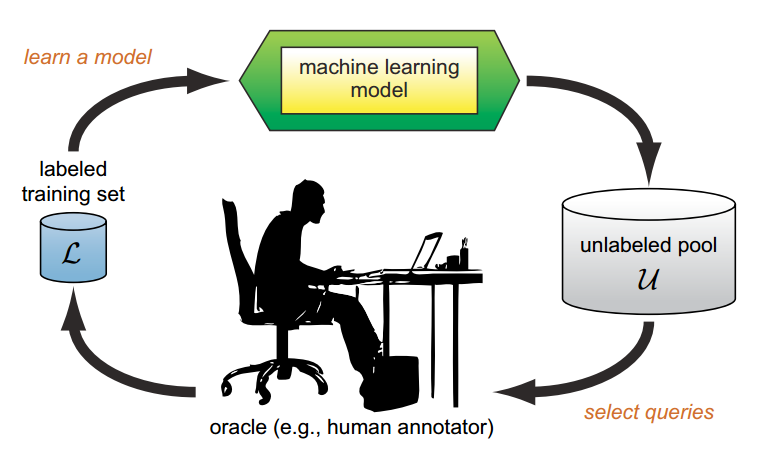
\includegraphics[width=\textwidth]{images/active_learning}
    \caption{Workflow of active learning \cite{Settles2010}.}
    \label{ac_workflow}
\end{figure}

Active learning seems to be the best choice for this task as it actively queries the human for grades of the samples it is most uncertain of. Fig \ref{ac_workflow} illustrates a typical workflow of active learning. Active learning is a subfield of machine learning which works under the hypothesis that if the learning algorithm is allowed to choose the data from which it learns it will perform better with less labeled data and training \cite{Settles2010}. Such a model queries a user / human expert for the labels of certain data samples in such a way that it can learn to produce the desired outputs with higher accuracy. By actively selecting the data samples to label, it reduces a considerable amount of labeled training samples, thus, alleviating the problem of insufficient labeled data which is prevalent in supervised learning approaches. In addition, it would be a solution to deal with the diversity in answers as there is generally no single best response for an open-ended question.   

\newpage
\section{Problem Statement}
\begin{itemize}   {\tiny }
\vspace*{1\baselineskip}
    \item One of the biggest challenge involved in supervised learning in the need for large labeled datasets. Generating a large data for short answer grading is also an obstacle. Many automatic short answer grading systems rely on supervised learning techniques. This, in turn, leads to high annotation cost of labeling the large training data. Also, the workload for labeling the data is more.
    \item As new data are generated on a regular basis, retraining the model for every new data also have a caveat of high computation cost.  Developing a generic model to overcome the deficit of retraining the model for every new answer can solve this issue.
    \item Short answer grading typically focuses on the content rather than the style of writing. Short answers written by students have a lot of lexical diversity. Active learning can be used to handle the lexical diversity by involving human in training the model.
\end{itemize}


\chapter{Related Work}

\section{Concept mapping based:}
	Concept mapping based techniques refers to splitting student answer into various concepts and graded based on the existence or non-existence of individual concepts\cite{Burrows2015}.
	
	\begin{itemize}
	 \item Callear et al.(2001) \cite{Callear2001}	developed a  computer-assisted assessment (CAA) termed as Automated Text Marker (ATM) in which the answers are  split  into  their  smallest  viable  unit  of concepts. All the atomic concepts are given some weight for the purpose of grading

	\item Leacock et al. (2003)\cite{Leacock2003} developed an automated scoring system called C-rater for ETS(Educational Testing Service) technologies to grade responses to content-based short answers based on the syntactical matching(subject, object, and verb). This uses deep natural language processing to determine the correctness of student responses. The preprocessing steps done by the c-rater systems include spelling correction, determining the grammatical structure of each sentence, resolving pronoun reference and analyzing paraphrases.
	
	  \item Brill et al. (2002) \cite{Brill2002} developed a question answering system called AskMSR. It uses the techniques such as query-reformulation, n-gram mining, filtering, and n-gram tiling. This system reformulates queries as declarative sentence segments to help query-answer matching. The shortcoming of this approach is that it works only when the (exact) content words appearing in a query appears also in the answer.
	
\end{itemize}


\section{Information extraction:}

	Information extraction system refers to 
extracting patterns from student answer followed by a series of pattern matching operations that includes regular expression or parse trees \cite{Burrows2015}.

\begin{itemize} 

	\item Bachman et al. (2002) \cite{Bachman2002} developed a short answer scoring system called WebLAS.  This system extracts regular expressions from a model answer to generate a scoring key. This grading system finds important segments of teacher answers through parsing and prompt the teacher to confirm the weights. It also prompts the teacher to confirm or decline the semantically similar alternatives.
	\item Mitchelle et al. (2002) \cite{Mitchell2002} discuss a software called AutoMark, which is developed to achieve robust grading of short answers for open-ended questions. This approach employs information extraction techniques to provide computerized marking of short free-text responses. Student answers are first parsed, and then intelligently matched against each mark scheme template, and a mark for each answer is computed. 
	\item Oxford UCLES is an information extraction short answer scoring system that was developed at the Oxford University.  which uses hand-crafted patterns by human experts to compare the answers with the model answer by Pulman et al. (2005) \cite{Pulman2005}. This work compares information extraction with both hand-crafted and machine learning assisted pattern matching.  The results of attempting to use machine learning strategies to extract patterns were not satisfactory.  It was concluded that hand-crafted patterns perform better than machine learned patterns. 
	\item Jordan and Mitchell (2009) \cite{Jordan2009} developed a graphical user interface(FreeText Author) for short answer grading whereby the teacher’s model answer is converted into syntactic-semantic templates for the student answers to be matched against. The question authors don’t have to be well versed in Natural Processing Techniques as the model creates the patterns from the correct answers by its own.
	\item Raheel Siddiqi (2010)\cite{Siddiqi2010} proposes a grading system that works on the structure of students' answer. It simply uses question answer markup language (QAML) to represent the required answer structures. The evaluation process starts with spell checking and some basic linguistic analysis, then the system matches the student’s answer text structure with the required saved structure to compute the final mark.
	\item Meurers et al. (2011) \cite{Meurers2011} and Hahn et al. (2012) \cite{Hahn2012} used semantic analysis to align student and target answers, including functional roles such as subject/object, gives better performance over similarity measures.
	\item Higgins et al. (2014) \cite{Higgins2014} work describe the importance and the efficiency of syntactically-informed features like n-gram features, language model features, dependency features, k-nearest neighbor features and discourse segment features in short answer grading.
    \item Ramachandran et al. (2015) \cite{Ramachandran2015} developed a short answer scoring system to provide effective scoring using automatic pattern extraction. Word-order graphs and semantic metrics(Lexico-semantic matching technique) were used to identify important patterns automatically from human-provided rubric texts and top-scoring student answers. Patterns were automatically extracted using two algorithms namely, generating patterns containing unordered content tokens and generating patterns containing sentence structure or phrase pattern information.
    
\end{itemize}

\section{Corpus based:}

Corpus-based methods are the statiscal methods that uses large document corpora(wikipedia, google etc.,) to obtain informations like synonyms, degree of similarity,frequency of term pairs etc. \cite{Burrows2015},

\begin{itemize}
	\item Mihalcea et al.,(2006) \cite{Mihalcea2006} found comparable results to corpus-based measures by using word-to-word similarity measures.
	\item Nielsen et al., (2009) \cite{Nielsen2009}proposed a dependency-based classification component called Intelligent Tutoring System. In this approach, the instructor answers are parsed, enhanced, and manually converted into a set of content-bearing dependency triples or facets. The system uses a decision tree trained on part-of-speech tags, dependency types, word count, and other features to attempt to learn how best to classify an answer/facet pair.
	 \item Mohler and Mihalcea (2009) \cite{Mohler2009} use the similarity between the students’ answers and the teacher’s answers for automatic short answer grading. This work addresses topics such as comparison of knowledge-based and corpus-based measures of text similarity, evaluation of the effect of domain and size on the corpus-based measures, and a novel technique to improve the performance of the system by integrating automatic feedback from the student answers. Eight knowledge-based measures of semantic similarity and two corpus-based semantic similarities for short answer grading were successfully compared. They also created a dataset of questions, students answers and the grades for those answers given by two human annotators. Making the dataset open-source contributed a lot to other researchers to benchmark their implementations on it.
	 \item Gomaa and Fahmy (2012) \cite{Gomaa2012} use string similarity and corpus-based similarity for automatic short answer grading. In addition to comparing different similarity measures, they compared the usefulness of two different corpora as well and this gave some insight into the useful features of a corpus. This work also reinforced the fact that short answer grading could be formulated as a similarity task.
	 
	\end{itemize}

\section{Machine learning:}

Machine learning based approaches refers to training a model utilizing the features extracted using  natural language processing techniques \cite{Burrows2015}.

\begin{itemize}
	\item Mohler et al. (2011) \cite{Mohler2011} like his previous approach uses the similarity between the students’ answers and the teacher’s answers for grading but incorporated several graph alignment features along with lexical semantic similarity measures This approach uses machine learning techniques and concludes that the student answers can be more accurately graded by incorporating the graph alignment features along with semantic measures. An attempt was also made to align the dependency graphs of the student and the instructor answers in order to make use of a structural component in the automatic grading of student answers.
	\item Fast, simple, and high-performance short answer grading system was proposed by Sultan et al. (2016) \cite{Sultan2016} that uses text similarity features such as word alignment, embeddings, question demoting, term weighting and length ratio was proposed. A supervised learning model is trained using this features to predict the grades for short answer grading.     
     
    \item Basu et al. (2013) \cite{Basu2013} developed an approach termed as Powergrading. This approach of divide and conquer the short answers proved to be useful in reducing the number of actions required for grading them by extending the impact of a small number of user actions when grading resources are limited. Their work incorporates clustering in short answer grading to cluster the similar answers together. This work gave an efficient solution to one of the main deficits of automated short answer grading, namely, capturing the modes of misunderstanding among the students’ answers.
    
\end{itemize}
    \newpage
    
The research in automatic short answer grading started as matching the concepts in students' answers to that of teacher's model answer and then moved on to match patterns such as regular expressions or parse tree which were written by experts (information extraction). Both of these methods could be categorized under rule-based methods which is best for repeated assessment. The latter part of the research focused into more statistical models such as corpus-based techniques (harnessing information from large corpora to calculate the degree of similarity) and machine learning techniques (features extracted form answers using Natural Language Processing techniques and machine learning models are used to compute the final grade). These models were found to work well for unseen questions and new domains \cite{Burrows2015}.

\vspace{5mm}

Requiring large amount of annotated dataset, inconsistent performance, lack of generic scoring models for new dataset, depending on a single best answer, and the need of a human expert's hand to write down the patters are some of the common drawbacks that were inherent in these works. In light of the aforementioned problems, evaluating active learnign for short answer grading would be the next best logical step. In \cite{Horbach2016}, the authors have investigated the applicability of active learning for this task and have presented a brief study on different methods of item selection, seed selection and the influence of different numbers of samples to be labeled at each iteration. In this research and development project, we strive to extend this step of applying active learning to short answer grading by exploring different techniques and algorithms in natural language processing and active learning. 



\chapter{Project Plan}

\section{Work Packages}
The bare minimum will include the following packages:
\begin{enumerate}
    \item[WP1] Problem formulation and proposal
    \begin{itemize}
    \item Problem formulation
    \item Proposal
    \end{itemize}
    \item[WP2] Natural language processing and active learning
    \begin{itemize}
    \item Understanding concepts
    \item Hands on Natural language processing tools and libraries
    \item Understanding active learning algorithms
    \end{itemize}
    \item[WP3] Literature survey
    \begin{itemize}
    \item Collect most relevant papers
    \item Shortlist papers that include computerized short answer grading
    \item Shortlist papers that include active learning in the context of NLP
    \end{itemize}
    \item[WP4] Working on datasets
    \begin{itemize}
    \item Reviewing existing datasets
    \item Compile new dataset
    \end{itemize}
	\item[WP5] Evaluating various NLP features
	\begin{itemize}
    \item Evaluating features based on semantic similarity
    \item Evaluating features based on entailment
    \item Evaluating features based on pattern matching
    \item Evaluating features based on lexical similarity
    \end{itemize}
	\item[WP6] Evaluating various active learning strategies
	\begin{itemize}
    \item Evaluating various query strategy frameworks
    \item Empirical analysis of active learning for short answer grading
    \end{itemize}
	\item[WP7] Implementation
	\begin{itemize}
    \item Minimum working model
    \item Testing and evaluating performance
    \item Improvements
    \end{itemize}
	\item[WP8] Developing graphical user interface(GUI)
	\begin{itemize}
    \item User research
    \item Design and protyping
    \item Evaluation
    \end{itemize}
	\item[WP9] Final Report
	\begin{itemize}
    \item Writing report
    \item First draft of the report
    \item Corrections in report
    \item Final report
    \end{itemize}
\end{enumerate}
%Keep in mind that depending on your project, you will probably need to add work packages that are more suited to your projects.



\section{Milestones}
\begin{enumerate}
    \item[M1] Comprehensive state of art
    \item[M2] Determining the best NLP features for short answer grading
    \item[M3] Determining the best active learning strategy
    \item[M4] Delivering a working model
    \item[M5] Incorporating model into an interface
    \item[M5] Report submission
\end{enumerate}
\newpage
\section{Project Schedule}
%Include a gantt chart here. It doesn't have to be detailed, but it should include the milestones you mentioned above.
%Make sure to include the writing of your report throughout the whole project, not just at the end.

%\begin{figure}[h!]
 %   \includegraphics[width=\textwidth]%{rnd_deliverable_timeline}
%    \caption{}
 %   \label{}
%\end{figure}



\begin{figure}[hbtp]
\caption{Gantt chart}
\centering
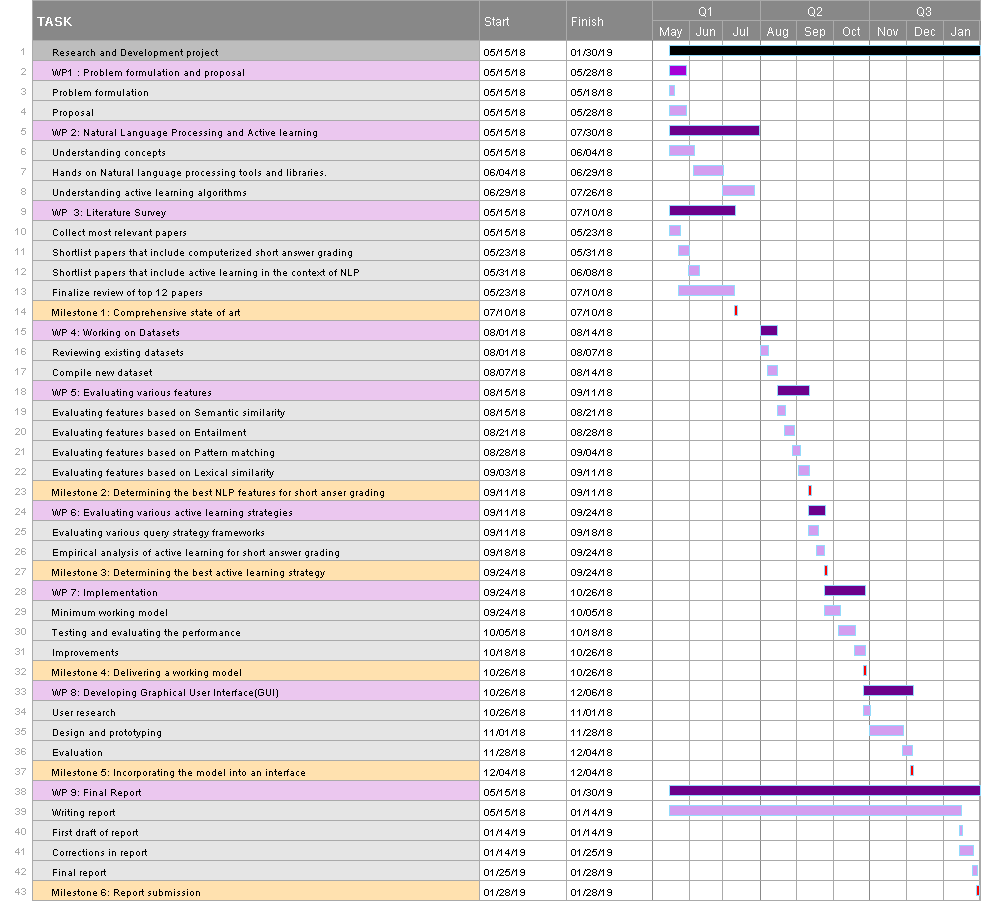
\includegraphics[scale=0.48]{images/gantt_chart.png}
\end{figure}

\newpage
\section{Deliverables}
\subsection{Minimum Viable}

\begin{itemize}
    \item Survey the existing approaches for computerized short answer grading
    \item Review existing datasets for automatic short answer grading.
    \item Compile new datasets from different in-house domain
\end{itemize}

\subsection{Expected}
\begin{itemize}
    \item Evaluate the quality of different features for interactive short answer grading
    \item Evaluate Active Learning strategies for Short-Answer grading
    \item Implement a working model of 100 clicks for 1000 grades.
\end{itemize}

\subsection{Desired}
\begin{itemize}
    \item Integrate the best model with a graphical user interface(GUI)
\end{itemize}


\nocite{*}




\bibliographystyle{plainnat} 
% Use the plainnat bibliography style
\bibliography{bibliography.bib} % Use the bibliography.bib file as the source of references
\end{document}
